
\pstart \footnotesize Redeundo jam ergo ad figuram 1. ponendoque pondus operculo (sive si mavis Embolo) \textit{AB} impositum, habere in quolibet \edtext{spatii puncto}{\lemma{quolibet}\Afootnote{ \textit{ (1) }\ spatio \textit{ (2) }\ spatii puncto \textit{ L}}} ut \textit{I} vel \textit{L} incrementa virium\protect\index{Sachverzeichnis}{incrementum!virium} ut reciproca applicatarum parabolae ad axem seu ut $\displaystyle \frac{1}{\surd y}$; at decrementa virium ut \edtext{\textit{y}}{\lemma{ut}\Afootnote{ \textit{ (1) }\ $\displaystyle \frac{y^2}{1}$ \textit{ (2) }\ earum \textit{ (3) }\ erit virium progressio \textit{ (4) }\ \textit{y} \textit{ L}}} seu ut rectas \textit{KN,} \textit{MP}. Erit progressio ex incrementis decrementisque composita, seu progressio mutationum, \edtext{ut}{\lemma{mutationum,}\Afootnote{ \textit{ (1) }\ ex \textit{ (2) }\ ut \textit{ L}}} $\displaystyle \frac{1}{\surd y}\smallfrown\frac{y}{1}\sqcap\frac{y}{\surd y}$, sive ut $\displaystyle\frac{\surd y^2}{\surd y}$, sive ut $\displaystyle\surd\frac{y^2}{y}$, sive ut $\displaystyle\surd y$, sive ut applicatae \edtext{parabolae ad axem}{\lemma{applicatae}\Afootnote{ \textit{ (1) }\ Hyperbolae ad axem \textit{ (2) }\ parabolae ad axem \textit{ L}}}. Error est non in se invicem duci sed a se invicem subtrahi debent: fiet scilicet $\displaystyle \frac{1}{\surd y}-\frac{y}{1}$, sive $\displaystyle\frac{1-y\surd y}{\surd y}\sqcap \omega$ unde $\displaystyle \frac{1-2y\surd y+y^3}{y}\sqcap \omega^3$, sive $\displaystyle\Box \llcorner \omega^2y-y^3-1\lrcorner \sqcap 4y^3$, sive $\displaystyle \omega^2y\sqcap 5y^3+1$ figura conchoeidis cuidam aut cissoeidis \edtext{momentis}{\lemma{}\Afootnote{momentis \textit{ erg.} \textit{ L}}} non absimilis. Homogeneam incremento virium\protect\index{Sachverzeichnis}{incrementum!virium} in 
%Zeitz auskommentiert \begin{wrapfigure}{l}{0.17\textwidth}                    
%                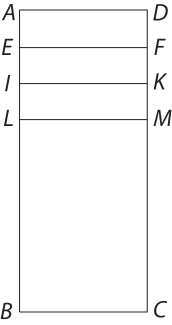
\includegraphics[width=0.17\textwidth]{images/35_5_6v}\\\rule[0cm]{0.6cm}{0cm}\textit{[Fig. 4]}
%                        %\caption{Bildbeschreibung}
%                        \end{wrapfigure}
%                        %@ @ @ Dies ist eine Abstandszeile - fuer den Fall, dass mehrere figures hintereinander kommen, ohne dass dazwischen laengerer Text steht. Dies kann zu einer Fahlermeldung fuehren. @ @ @ \\
                        dicta fig. 1. quod incrementum, decremento tandem vinci manifestum est, tunc scilicet cum \textit{y} fit $\raisebox{0.8pt}{$\urcorner$} \hspace{-5.5pt}|\hspace{3pt}$ quam 1. Sed jam suspicari incipio in figura 1. adjectaque ei ratiocinatione egregie a me erratum esse. Nimirum si vis compressionis\protect\index{Sachverzeichnis}{vis!compressionis} usque in \textit{M}, esset ad vim compressionis\protect\index{Sachverzeichnis}{vis!compressionis} 
usque in \textit{F}, ut \textit{DMP} ad \textit{DFH}. 
Sequeretur vi quae sit finita seu ad datam assignabilem, ut Triangulum \textit{DCG} ad aliud v.g. ad \textit{DMP} comprimi posse aerem in spatium infinite parvum seu quod idem est annihilari, quod est absurdum. Longe alia ergo ratione calculandum est. 
Pone aerem \edtext{spatium \textit{ABCD} naturaliter implentem esse}{\lemma{aerem}\Afootnote{ \textit{ (1) }\ esse \textit{ (2) }\ spatium \textit{ABCD} naturaliter implentem esse \textit{ L}}} \textit{ab}\edtext{. Ponendo}{\lemma{\textit{ab}}\Afootnote{ \textit{ (1) }\ portionem ejus infinite parvam esse \textit{ (2) }\ . Ponendo \textit{ L}}} \textit{AB} $\sqcap$ \textit{a}, et \textit{BC} $\sqcap$ \textit{b}, sit \textit{AE} \edtext{$\sqcap$ \textit{y} fiet \textit{AEFD} $\sqcap$ \textit{yb}}{\lemma{\textit{AE}}\Afootnote{ \textit{ (1) }\ infinite parva, $\sqcap$  \textit{(a)}\ $\beta$ \textit{(b)}\ $\gamma$ \textit{ (2) }\ $\sqcap$ \textit{y} fiet \textit{AEFD} $\sqcap$  \textit{(a)}\ $\gamma$ \textit{b} \textit{(b)}\ \textit{yb} \textit{ L}}}\edtext{. Resistentia}{\lemma{\textit{yb}}\Afootnote{ \textit{ (1) }\ eodem ergo aere intra spatium \textit{EF}   \textbar\ compresso \textit{ erg.}\ \textbar\  erit vis aeris qua Elaterio\protect\index{Sachverzeichnis}{elaterium|textit} seu compressioni resistit, ut $\gamma b$ divisa per \textit{ab} seu ut $\displaystyle\frac{\gamma}{a}$ \textit{ (2) }\ . Resistentia \textit{ L}}} ergo erit tanta, quantum invenit aer $\gamma b$ seu spatii \textit{AEFD}, distribuendus per omnia puncta spatii \textit{EBCF}. \edtext{Aestimanda}{\lemma{\textit{EBCF}.}\Afootnote{ \textit{ (1) }\ Quae \textit{ (2) }\ Aestimanda \textit{ L}}} ergo quantitas resistentiae tum a magnitudine aeris \textit{AEFD}, tum a parvitate spatii \textit{EBCD}, tum a \edtext{magnitudine}{\lemma{a}\Afootnote{ \textit{ (1) }\ quantitate \textit{ (2) }\ magnitudine \textit{ L}}} resistentiae quae in singulis hujus spatii punctis reperitur. Magnitudo aeris \textit{AEFD} $\sqcap$ $\gamma b$; magnitudo spatii est \textit{EBCF}, est $ab-yb$. Ponendo \textit{AE} $\sqcap$ \textit{y}, \edtext{resistentia puncti aeris}{\lemma{resistentia}\Afootnote{ \textit{ (1) }\ in quoli \textit{ (2) }\ aeris in \textit{ (3) }\ puncti aeris \textit{ L}}} \edtext{in statu ordinario positi ad recipiendum}{\lemma{aeris}\Afootnote{ \textit{ (1) }\ ad recipiendum \textit{ (2) }\ in [...] recipiendum \textit{ L}}} aliud punctum aeris sibi aequale ponatur esse \textit{d}. Resistentia ergo aeris in spatio $ab-yb$ ad recipiendum aeris tantundem est \edtext{$abd-ybd$}{\lemma{est}\Afootnote{ \textit{ (1) }\ \textit{ab$\delta$\textendash yb$\delta$} \textit{ (2) }\ $abd-ybd$ \textit{ L}}} \edtext{quae est ad resistentiam}{\lemma{$abd-ybd$}\Afootnote{ \textit{ (1) }\ . Ergo resistentia \textit{ (2) }\ quae est ad resistentiam \textit{ L}}} \edtext{ejusdem}{\lemma{}\Afootnote{ejusdem \textit{ erg.} \textit{ L}}} aeris in spatio \textit{EBCF} \edtext{quaesitam}{\lemma{quaesitam}\Afootnote{ \textit{ erg.} \textit{ L}}} ad recipiendum aerem spatii \textit{AEFD}, ut spatium \textit{AEFD}, ad \edtext{spatium}{\lemma{ad}\Afootnote{ \textit{ (1) }\ aerem \textit{ (2) }\ spatium \textit{ L}}} \textit{EBCF}, seu ut \edtext{$ab-yb$ ad \textit{yb}}{\lemma{ut}\Afootnote{ \textit{ (1) }\ \textit{yb} ad \textit{ (2) }\ $ab-yb$ ad \textit{yb} \textit{ L}}} seu ut \textit{y} ad \edtext{$a-y$. $\displaystyle\frac{Resistentia\hspace{5.5pt}ergo\hspace{5.5pt}quaesita}{abd-ybd}\sqcap\frac{y}{a-y}$.
 % \begin{wrapfigure}{l}{0.4\textwidth}                    
                %\includegraphics[width=0.4\textwidth]{../images/Schediasma+de+calculo+elastico/LH035%2C05%2C02_006v/files/100487.png}
                        %\caption{Bildbeschreibung}
                        %\end{wrapfigure}
                        %@ @ @ Dies ist eine Abstandszeile - fuer den Fall, dass mehrere figures hintereinander kommen, ohne dass dazwischen laengerer Text steht. Dies kann zu einer Fahlermeldung fuehren. @ @ @ \\
                    }{\lemma{$a-y$.}\Afootnote{ \textit{ (1) }\ Resistentia ergo \textit{ (2) }\ $\displaystyle\frac{abd-ybd}{quaesita}\sqcap$ \textit{ (3) }\ $\displaystyle\frac{Resistentia\hspace{5.5pt}ergo\hspace{5.5pt}quaesita}{abd-ybd}\sqcap\frac{y}{a-y}$ \textit{ L}}}\rule[-4mm]{0mm}{10mm} Ergo resistentia quaesita aeris scilicet naturalis in spatio \textit{EBCF}, ad recipiendum aerem spatii \textit{AEFD}, etiam naturalem, erit $\sqcap$ \edtext{\textit{ybd}}{\lemma{$\sqcap$}\Afootnote{ \textit{ (1) }\ \textit{y} $\sqcap$ \textit{ (2) }\ \textit{ybd} \textit{ L}}} ut patet; \edtext{sed quia progressu temporis locive fit, ut aer}{\lemma{patet;}\Afootnote{ \textit{ (1) }\ sed si aer \textit{ (2) }\ sed [...] aer \textit{ L}}} non maneat in statu naturali, sed ut intrudendus pariter et recipiens sint jam tum plurimum compressi, ideoque aliter \edtext{longe}{\lemma{aliter}\Afootnote{ \textit{ (1) }\ paulo \textit{ (2) }\ longe \textit{ L}}} instituendus est calculus.
                    \pend 
                    \pstart 
                    \footnotesize Nimirum recta \textit{AB} divisa intelligatur in partes aequales infinite parvas \textit{AE}, \textit{EI}, \textit{IL}, etc.  $\sqcap$ $\gamma$ \edtext{aer}{\lemma{$\gamma$}\Afootnote{ \textit{ (1) }\ spatium \textit{ (2) }\ aer \textit{ L}}} \textit{AEFD} erit $\sqcap$ $\gamma b$. \edtext{Jam $\lambda$}{\lemma{Jam}\Afootnote{$\lambda$ \textit{ erg.} \textit{ L}}} resistentia aeris \textit{EBCF} ad eum recipiendum; est ad \edtext{$ab\delta-\gamma b\delta$ (factum ex ductu $\delta$, resistentiam cujuslibet puncti aerei ad recipiendum sibi aequale in spatium $ab-\gamma b$) seu ad}{\lemma{$ab\delta-\gamma b\delta$}\Afootnote{ [...] seu ad \textit{ erg.} \textit{ L}}} resistentiam \edtext{aeris \textit{EBCF}}{\lemma{resistentiam}\Afootnote{ \textit{ (1) }\ ipsius \textit{EBC} \textit{ (2) }\ aeris \textit{EBCF} \textit{ L}}}, ad recipiendum aerem sibi aequalem, ut \textit{AE} $\sqcap$ $\gamma$, ad \textit{EB} $\sqcap \hspace{3pt}a-\gamma$ seu $\lambda \sqcap \gamma b\delta$ intruso jam aere \textit{AEFD} in spatium $EBCF$. Erit jam aer spatii \textit{EBCF} \edtext{\textit{ab$\delta$}}{\lemma{\textit{EBCF}}\Afootnote{ \textit{ (1) }\ (nominando quodlibet ejus punctum $\delta$) $\sqcap$ \textit{ (2) }\ \textit{ab$\delta$} \textit{ L}}}, loco $ab\delta-\gamma b\delta$ ac proinde ut est \textit{ab$\delta$} ad $ab\delta-\gamma b\delta$, ita erit $b\gamma\mu$ aer spatii \textit{EIKF} (post intrusionem aeris \textit{AEFD}, in spatium \textit{EBCF}) ad $b\gamma \delta$ \edtext{aerem}{\lemma{$b\gamma \delta$}\Afootnote{ \textit{ (1) }\ resistentiam aeris \textit{ (2) }\ aerem \textit{ L}}} spatii aequalis sed\edtext{}{\lemma{}\Afootnote{sed  \textbar\ non \textit{ gestr.}\ \textbar\ compressione \textit{ L}}} compressione carentis \textit{AEFD}, ergo resistentia aeris in spatio \textit{EIKF}, seu $\displaystyle \mu \sqcap\frac{ab\delta}{ab-\gamma b}\sqcap\frac{a\delta}{a-\gamma}$
                   % @@@ G R A F I K @@@% \begin{wrapfigure}{l}{0.4\textwidth}                    
                %\includegraphics[width=0.4\textwidth]{../images/Schediasma+de+calculo+elastico/LH035%2C05%2C02_006v/files/100740.png}
                        %\caption{Bildbeschreibung}
                        %\end{wrapfigure}
                        %@ @ @ Dies ist eine Abstandszeile - fuer den Fall, dass mehrere figures hintereinander kommen, ohne dass dazwischen laengerer Text steht. Dies kann zu einer Fahlermeldung fuehren. @ @ @ \\
                    . \edtext{}{\lemma{$\displaystyle\frac{a\delta}{a-\gamma}$}\Afootnote{.  \textbar\ Itaque si jam  \textit{streicht Hrsg.}\ \textbar\ Porro \textit{ L}}}\edtext{Porro aer \textit{EIFK} compressus seu}{\lemma{$\displaystyle\frac{a\delta}{a-\gamma}$.}\Afootnote{ \textit{ (1) }\ Eadem porro ratione,  \textit{(a)}\ intruso aere \textit{EIFK}, id est aere \textit{AIKD}, id est aere 2 $\gamma b\delta$ \textit{(b)}\ si aer \textit{EIFK}, compressus, id est aer \textit{AIKD} naturalis, qui ad aerem \textit{IBCK}, compressum $\sqcap$ $ab\delta$, est  \textit{(aa)}\ ut \textit{IK} $\sqcap$ $\gamma$ ad \textit{(bb)}\ ut \textit{EI} $\sqcap$ $\gamma$ ad \textit{IB} $\sqcap$ $a-2\gamma$ et qui proinde est $\displaystyle\sqcap\frac{ab\delta\gamma}{a-}$ \textit{ (2) }\ Porro aer \textit{EIFK} compressus seu \textit{ L}}} $\mu b\gamma$, seu $\displaystyle\frac{ab\delta\gamma}{a-\gamma}$ in aerem \textit{IBCK}, qui est $\mu, \smallfrown a-\gamma, \smallfrown b,$ seu $\displaystyle\frac{a\delta}{a-\gamma}, \smallfrown a-2\gamma, \smallfrown b$ intrudendus sit tunc in spatio $a-2\gamma, \smallfrown b$ habebitur aer totus qui antea fuit \textit{ABCD}, nempe 
                    \edtext{\textit{ab$\delta$}: [5 r\textsuperscript{o}] }{\lemma{\textit{ab$\delta$}:}\Afootnote{ \textit{ (1) }\ Et vis \textit{ab$\delta$} \textit{ (2) }\  Brevius ergo ita ratiocinabimur: primum aer omnis: \textit{abe} implet spatium \textit{ABCD} $\sqcap$ \textit{ab} postea idem aer \textit{abe} implet spatium $a-\gamma, \smallfrown b \sqcap EBCF$  \textit{(a)}\ resistentiam aeris \textit{(b)}\ vim   \textit{(aa)}\ aeris ad \textit{(bb)}\ puncti aeris, \textit{e} resistendum  \textit{(aaa)}\ potentiae aequ \textit{(bbb)}\ compressioni in spatium dimidium, seu ad recipiendum aeris tantundem, vocemus $\delta$, erit \textit{r}  \textit{(3)}\ Brevius ita ratiocinabimur: \textit{(4)}\ Esto \textit{ L}}} Esto \edtext{spatium cylindricum}{\lemma{Esto}\Afootnote{ \textit{ (1) }\ spatium cyli \textit{ (2) }\ recta \textit{ (3) }\ spatium cylindricum \textit{ L}}} sive prismaticum,  
\edtext{cujus sectio}{\lemma{prismaticum}\Afootnote{ \textit{ (1) }\ \textit{ABCD} \textit{ (2) }\ , cujus sectio \textit{ L}}} a plano facta basi \edtext{perpendicularis, rectangulum \textit{ABCD}}{\lemma{perpendicularis,}\Afootnote{ \textit{ (1) }\ \textit{ABCD} \textit{ (2) }\ rectangulum \textit{ABCD} \textit{ L}}}, quod considerare suffecerit \edtext{cum eadem omnia in Solido intelligi possint}{\lemma{cum [...] possint}\Afootnote{\textit{ erg.} \textit{ L}}}. 
Recta \textit{AB} esto \textit{b}, recta \textit{BC}, \textit{c}. Punctum quodlibet aeris vocetur $\alpha$ et vis qua punctum aeris resistit alterius puncti aeris sibi aequalis in spatium suum receptione, seu compressione\protect\index{Sachverzeichnis}{compressio} sui ex spatio naturali in dimidio angustius, vocetur $\delta$. Aer spatii \textit{ABCD} erit \textit{bc}$\alpha$. Esto linea rigida in \textit{AD}, basi \textit{BC} parallela, quae promoveatur situ \textit{AD} in situm \textit{EF}, aeremque \textit{AEFD} \edtext{intrudat in spatium}{\lemma{intrudat}\Afootnote{ \textit{ (1) }\ ex spatio \textit{ (2) }\ in spatium \textit{ L}}} \textit{EBCF}. Recta \textit{AE} vocetur \textit{y}. Jam per media rectarum \textit{AB}, \textit{DC} puncta transeat recta \textit{GH}. Manifestum est ex Hypothesi, vim quam habeat aer omnis \edtext{\textit{ABCD}}{\lemma{}\Afootnote{\textit{ABCD} \textit{ erg.} \textit{ L}}} in spatium \textit{GBCH} compressus esse \textit{bc}$\alpha$$\delta$. Quoniam ita erit ut quodlibet ejus punctum dimidium occupet spatium situs naturalis.
\pend 